\documentclass[12pt,a4paper]{article}
\usepackage[german]{babel}
\usepackage{mathptmx, amsmath}
\usepackage[utf8x]{inputenc}
\usepackage[boxruled]{algorithm2e}

\usepackage{anysize}
\marginsize{30mm}{30mm}{15mm}{15mm}	
 
\usepackage{epsfig}	

\usepackage{fancyhdr}
\pagestyle{fancy}
\fancyhead{}
\fancyhead[L]{\small{The necessity for natural conversation with virtual agents}}
\fancyhead[C]{\small{}}
\fancyhead[R]{\small{Jan Pöppel}}
\renewcommand{\headrulewidth}{0pt}

\usepackage{wrapfig}
\usepackage{color}
\usepackage[usenames,dvipsnames]{xcolor}
\usepackage{hyperref}

\begin{document}

\title{\bf{AsapBMLFlowVisualisation}}
\date{\today}
\author{Jan Pöppel \\[3mm]
{\tt jpoeppel@techfak.uni-bielefeld.de}}
\maketitle\thispagestyle{empty}

\section*{Quickstart}

From \textbf{AsapReaizerDemo/java/resource/} run \\
\textbf{go.bmlflowvisualizer} 
~\\~\\
Spread needs to be running for the BMLFlowVisualizer to work.
Basic information about the programm and it's functionality can be found under the 
Info menu (Menu $\rightarrow$ Info).

\tableofcontents

\section{Overview}

The BMLFlowVisualizer is a tool designed to visualise the bml flow in a running Asap environment. It allows the user to see what kind of bml blocks are send over 
ipaaca at what time. The bml blocks can alse be inspected to view their messages. 
Furthermore the user gets information about the current scheduling state of already recieved bml blocks. 

\subsection{Functionality}

This tool is supposed to make it easier to understand and debug the bml flow in an Asap environment. To that end, the bml blocks are shown in their temporal context as well
as in the context of their connections (see section \ref{sec:mainWin} for details). More detailed information about a certain bml block can be browsed by opening
the BML Information Window (see section \ref{sec:bmlinfo}) by double clicking a block in any of the visualisations. Furthermore it is possible to search for a specific
block using the search window (\ref{sec:search}). A recorded session can also be stored and loaded at a later time using the \textit{Save} and \textit{Load} options, 
provided by the menu or their respective shortcuts $CTRL+S$ and $CTRL+L$. A short summary about the different colours (see section \ref{sec:colours} for more detailes) 
and the basic functionality of the tool can be viewed using the Information Window, accessible using the menu button \textit{Info} or the shortcut $CTRL+I$.

\section{Details}

This section gives more detailed information about the different windows and the meaning behind the block colours.

\subsection{Main Window \label{sec:mainWin}}
Figure \ref{fig:overview} shows the main window of the BMLFlowVisualizer. The left half of the window visualises the history of the current Asap session, while the right
half visualises more detailed information about the current time. The red line on the left (as well as the number in the textbox below) 
indicates the current time, which detailed visualisation can be seen on the right half. 

The history section is basically seperated into 3 subsections. The top subsection visualises the blocks in their planning phase (submitted and in preperation).
The second subsection visualises the blocks in their scheduling phase (pending and lurking). The last subsection shows the blocks in their execution phase 
(e.g. in\_exec and done). All blocks should go through all three phases and be represented in each of them. The width of each block visualises the time 
the block has spend in its three phases (planning, scheduling and execution). 

The detailed section consist of two panels. The top panel visualises the bml blocks that are currently being planned, while the lower one visualises the blocks that are 
currently being scheduled and playing. It also shows their relative connection to each other. A dotted line between two blocks means that they have an \glqq append\grqq connection
while a complete line means that they have a \glqq chunk\grqq connection. In the detailed section the block width has no special meaning.

\begin{figure}[H!]
\centering
 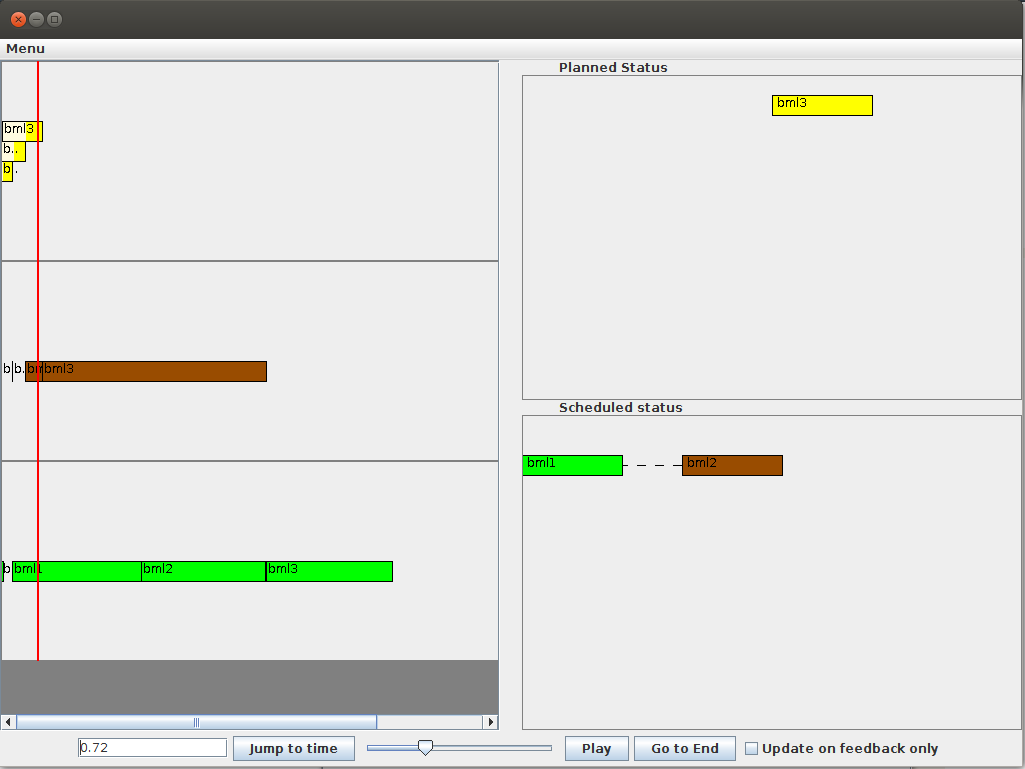
\includegraphics[width=\textwidth]{images/bmlFlowOverview.png}
 \caption{Main window of the BMLFlowVisualizer. The left half visualises the time history of the current session, while the right half shows more detailed information
 about the current timestep. The red line on the left symbolises the current time.}
 \label{fig:overview}
\end{figure}

\subsection{Search Window \label{sec:search}}

\subsection{BML Information Window \label{sec:bmlinfo}}

\subsection{Block colours \label{sec:colours}}




\end{document}